\newpage
\section{Komponenten}\label{sec:komponenten}
Für den Aufbau des Versuchs werden verschiedene Komponenten verwendet.
Im folgenden Kapitel werden diese vorgestellt:

\paragraph{Sony Playstation 4 \cite{PS4Welco38:online}}
Die \ac{ps4} ist eine Spielekonsole der aktuellen Generation.

\begin{figure}[h!]
    \centering
    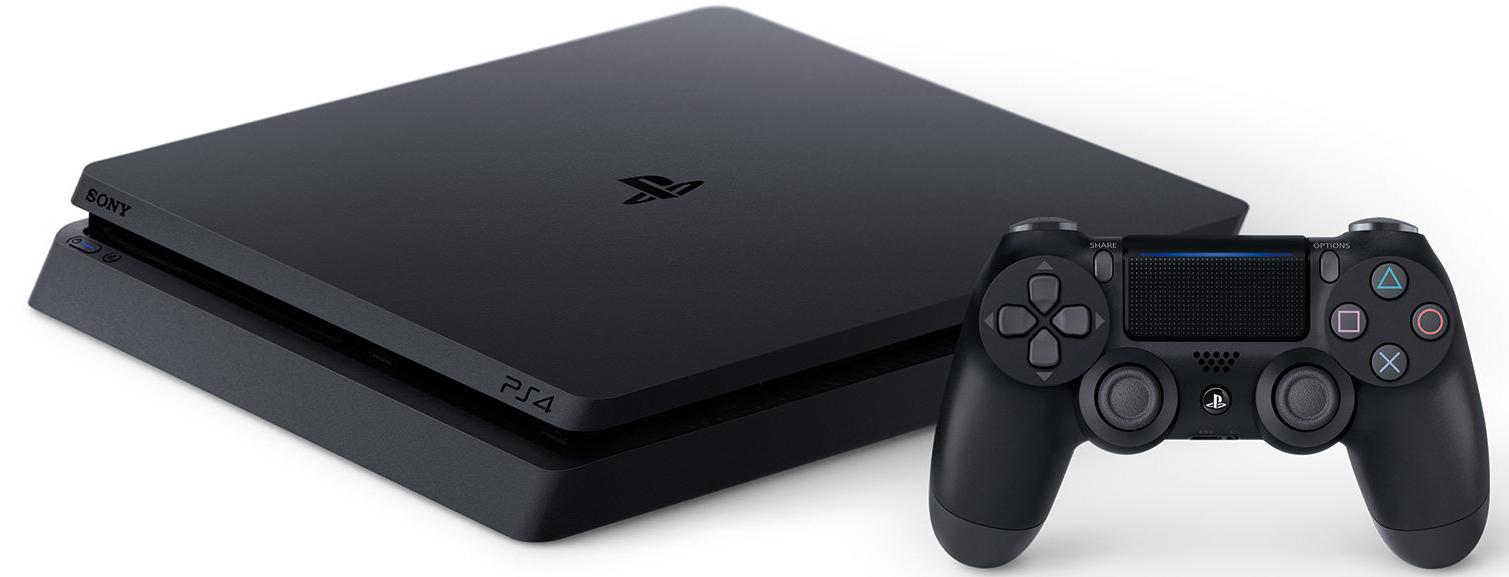
\includegraphics[width=0.4\textwidth]{ps4}
    \caption{Playstation 4 mit Controller}\label{fig:ps4}
\end{figure}

Gesteuert wird sie in der Regel durch einen Controller,
welcher hauptsächlich für Spiele konzipiert wurde.
Alternativ können auch diverse Bluetooth-Geräte oder eine Smartphone-App genutzt werden.

\paragraph{Raspberry Pi \cite{Whatisth47:online}}
Der Raspberry Pi ist ein weit verbreiteter Einplatinencomputer.
In diesem Projekt wird das Modell \textit{Raspberry Pi 3 Model B} verwendet.

\begin{figure}[h!]
    \centering
    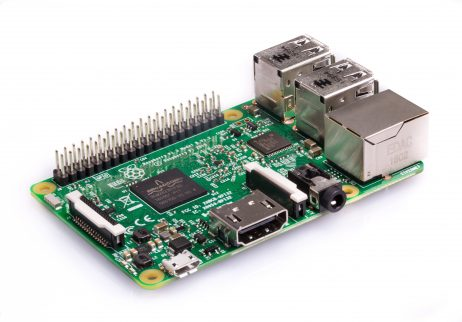
\includegraphics[width=0.4\textwidth]{pi}
    \caption{Raspberry Pi 3 Model B \cite{Raspberr2:online}}\label{fig:pi}
\end{figure}

Das offiziell unterstütze Betriebssystem ist \textit{Raspbian},
welches auf dem Linux-Betriebssystem \textit{Debian} basiert.
Alternativ können auch andere Betriebssysteme installiert werden,
welche besser auf einen bestimmten Anwendungsfall zugeschnitten sind.

\newpage

\paragraph{Home Assistant \cite{HomeAssi51:online}}
Home Assistant ist eine open-source Plattform zur Heimautomatisierung.
Basierend auf der Programmiersprache \textit{Python} ist sie dafür konzipiert
auf einem Raspberry Pi ausgeführt zu werden.
Mit \textit{Hassbian} wird ein Betriebssystem basierend auf \textit{Raspbian} angeboten,
auf welchen Home Assistant bereits installiert und konfiguriert ist.

\begin{figure}[h!]
    \centering
    
\includegraphics[width=0.2\textwidth]{homeassistant}
    \caption{Logo Homeassistant}\label{fig:homeassistant}
\end{figure}

Die Plattform ermöglicht das Überwachen und Steuern verschiedener Geräte zur Heimautomatisierung.
Für dieses Projekt wird der Home Assistant so konfiguriert,
dass er den Status der Playstation 4 überwacht und das Ein- bzw. Ausschalten ermöglicht.
Details zu dieser Konfiguration finden sich in Kapitel \ref{sec:aufbau} \textit{\nameref{sec:aufbau}}.

\paragraph{Logitech Harmony \cite{HarmonyH15:online}}
Logitech Harmony ist die Fernbedienungs-Sparte von Logitech.
In diesem Projekt wird der Harmony Hub zusammen mit der zugehörigen Harmony Elite Fernbedienung verwendet.
Durch den Harmony Hub könne zahlreiche Geräte über Infrarot, WLAN oder Bluetooth gesteuert werden.
Die Fernbedienung selbst kommuniziert hierbei über Funk \cite{HowToPoi90:online} mit dem Hub.
Der Hub gibt die Befehle an die entsprechenden Geräte weiter.

\begin{figure}[h!]
    \centering
    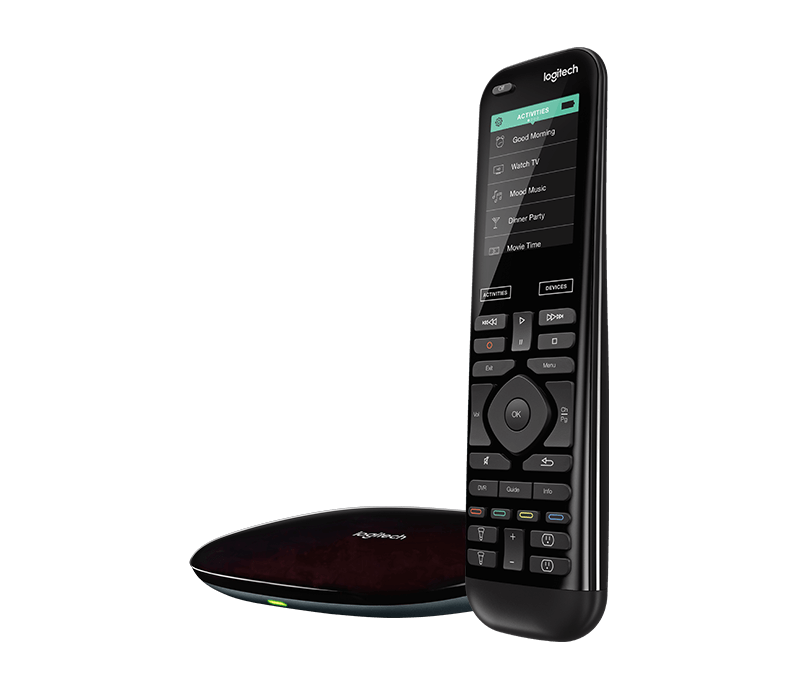
\includegraphics[width=0.3\textwidth]{harmony-elite}
    \caption{Harmony Hub mit Fernbedienung}\label{fig:harmony}
\end{figure}

Neben den verschiedenen Verbindungsmöglichkeiten ist ein großer Vorteil das Konfigurieren von \enquote{Aktionen}.
Diese sind eine Kombination von Befehlen an verschiedene Geräte.
So kann beispielsweise durch einen einzigen Tastendruck sowohl die Playstation 4,
als auch der Fernseher eingeschaltet werden.